\documentclass[../../../OAE-SPEC-MAIN.tex]{subfiles}
\begin{document}


\newpage
\section{RISC Protocol Design: OPCODE (Information)}\label{sec:opcode-information}

\begin{marginfigure}
 \centering
  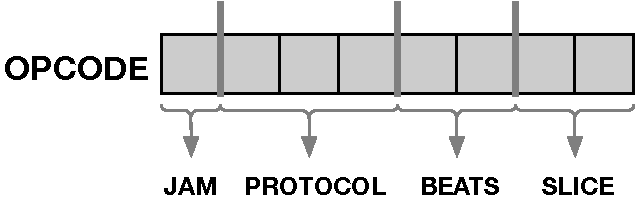
\includegraphics[width=1.1\linewidth]{./figures/opcode.pdf}
\caption{\centering One Byte Provides the entry point for  an Entire family of  Protocols}
\end{marginfigure}

\subsection{CONTEXT Frame format: First Slice, First Byte: OPCODE}

\begin{margintable}
%  \centering
  \footnotesize
  \rule{5.4cm}{0.8pt}\\
  \begin{tabular}{@{}cl@{}}
    \textbf{8SLICE} & \texttt{11 — TX Sender Init} \\
                   & \texttt{11 — RX SACK 1 (8B)} \\
                   & \texttt{10 — RX SACK 2 (16B)} \\
                   & \texttt{01 — RX SACK 3 (32B)} \\
                   & \texttt{00 — RX SACK 4 (64B)} \\
  \end{tabular}\\
  \rule{5.4cm}{0.6pt}
\end{margintable}

\begin{margintable}
  \footnotesize
  \rule{5.4cm}{0.8pt}\\
  \begin{tabular}{@{}cl@{}}
    \textbf{4SLICE} & \texttt{10 — TX Sender Init} \\
                      & \texttt{10 — RX SACK 3 (32B)} \\
                   & \texttt{01 — RX SACK 1 (8B)} \\
                   & \texttt{00 — RX SACK 2 (16B)} \\
  \end{tabular}\\
  \rule{5.4cm}{0.6pt}
\end{margintable}

\begin{margintable}
%  \centering
  \footnotesize
  \rule{5.4cm}{0.8pt}\\
  \begin{tabular}{@{}cl@{}}
    \textbf{2SLICE} & \texttt{01 — TX Sender Init} \\
                   & \texttt{01 — RX SACK 1 (8B)} \\
                   & \texttt{00 — RX SACK 2 (16B)} \\
  \end{tabular}\\
  \rule{5.4cm}{0.6pt}
\end{margintable}

\begin{margintable}
  \footnotesize
  \rule{5.4cm}{0.8pt}\\
  \begin{tabular}{@{}cl@{}}
    \textbf{1SLICE} & \texttt{00 — TX Sender Init} \\
                   & \texttt{00 — RX SACK 1 (8B)} \\
  \end{tabular}\\
  \rule{5.4cm}{0.6pt}
\end{margintable}

\begin{margintable} %  MAKE SPACE IN THE MARGIN
%  \centering
  \footnotesize
%  \rule{5.4cm}{0.8pt}\\
  \begin{tabular}{@{}cl@{}}
  \end{tabular}\\
%  \rule{5.4cm}{0.6pt}
\end{margintable}

\begin{margintable}
  \footnotesize
  \rule{5.4cm}{0.8pt}\\
  \begin{tabular}{@{}cl@{}}
    \textbf{BEATS} & \texttt{00 — TX 1 FRAME (64B)} \\
                   & \texttt{01 — TX 4 FRAMES (256B)} \\
                   & \texttt{10 — TX 16 FRAMES (1024B)} \\
                   & \texttt{11 — TX 64 FRAMES (4096B)} \\[3pt]
                   & \texttt{00 — RACK 1 FRAME (64B)} \\
                   & \texttt{01 — RACK 4 FRAMES (256B)} \\
                   & \texttt{10 — RACK 16 FRAMES (1024B)} \\
                   & \texttt{11 — RACK 64 FRAMES (4096B)} \\
  \end{tabular}\\
  \rule{5.4cm}{0.6pt}
\end{margintable}

\begin{margintable}
  \centering
  \footnotesize
  \rule{5.4cm}{0.8pt}\\
  \begin{tabular}{@{}cl@{}}
    \textbf{PROTOCOL} & \texttt{000 — Initialization} \\
                      & \texttt{001 — Liveness} \\
                      & \texttt{010 — State Machines} \\
                      & \texttt{011 — RESERVED} \\
                      & \texttt{100 — RESERVED} \\
                      & \texttt{101 — RESERVED} \\
                      & \texttt{110 — RESERVED} \\
                      & \texttt{111 — ESCAPE} \\
  \end{tabular}\\
  \rule{5.4cm}{0.6pt}
\end{margintable}

\begin{margintable}
  \centering
%  \vspace{1pt} % Trying to nudge down the table 
  \footnotesize
  \rule{5.4cm}{0.8pt}\\
  \begin{tabular}{@{}cl@{}}
    \textbf{JAM} & \texttt{ABORT/CANCEL} \\
  \end{tabular}\\
  \rule{5.4cm}{0.6pt}
\end{margintable}

(SLICE, BEATS, PROTOCOL, JAM) provides state encodings for an ultra-low-latency, hardware-friendly, and atomic transaction-friendly \AE thernet protocol.

Supports transactional operations, structured acknowledgments, and reversible flow control (causal backpropagation). Instead of positive-only credits, the first hop receiver provides the equivalent of negative credits, to indicate it is returning previously sent frames. %This is the first  level of reversibility. 

\subsection{nSLICE}
\marginnote{On cables shorter than the occupation time on the wire, slice acknowledges are sent  before the receiver sees the whole frame   --  exploiting full concurrency on the transmit/receive channels.}

\begin{description}
\item [Set by the Sender] to\texttt{[00]} --  indicating a  new context.
\item [Modified by the receiver] Closing the loop: \texttt{[11]$\rightarrow$[10]$\rightarrow$[01]$\rightarrow$[00]} %\footnote{In Bob Metcalfe's language} 
\end{description}

Encodes how many slices of the sender’s 64-byte Frame has been received so far. A 2-bit field with reversed temporal direction to encode the acknowledgment depth in a power of 2 \emph{number of slices}. This might represent the trailing edge of a window in a reversible or partially committed state machine. The naming “SACK”  suggests  slot or slice acknowledgments, as fine-grained positions in the interaction. 

%Note: We appear to be overloading 00 for both TX Sender Init and RX SACK 4 — this could be context-sensitive (e.g., distinguished by direction or PROTOCOL code).

\subsection{BEATS}

\sidenote{Encodes burst sizes TX (forwardproagation) and RX (backpropagation) code to frame groupings, enabling optimization of bandwidth and latency trade-offs.}

Defines a beat-structured flow control mechanism.  Sender declares the number of frames it plans to send advance. The receiver responds with a corresponding "slot acknowledgment".  Aimed at reliable, ordered delivery without the need for heavyweight TCP.


\subsection{PROTOCOL}

This field defines the high-level intent of the frame or transaction, by the sender (causal initiator). The 3-bit code is always in the first (context) slice of the Frame. Three of the eight possibilities are defined in this specification. The remaining ones are reserved for higher level protocols in this standard.  Escape will always be available to escape to legacy protocols. This compact opcode space (3 bits) is similar to what RISC architectures do. This simplifies logic at the NIC or SmartNIC level and allows for deterministic dispatch.
%\marginnote{ STUFF }

\subsection{PRE-EMPT/JAM}

\sidenote{The use of “JAM” evokes classic Ethernet collision handling, but here it's modernized for transactional cancellation or rollback.}

\nopagebreak[2]Set by TX to \texttt{[0]}. Set by RX to \texttt{[0]} to accept, and  \texttt{[1]} to pre-empt, for error, or to (cancel/rollback the transaction).


\end{document}
